\documentclass{standalone}
\begin{document}
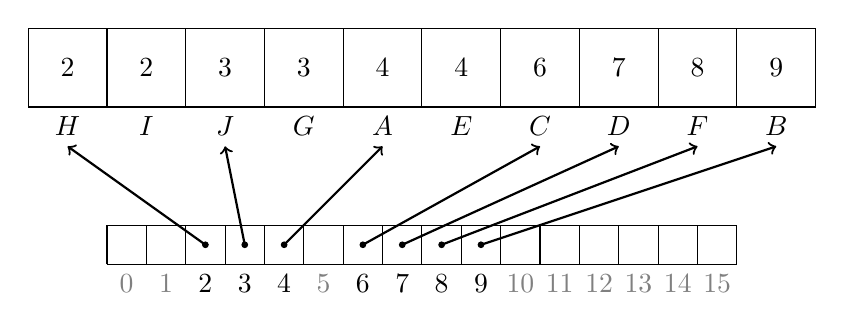
\begin{tikzpicture}

\draw (0, 0) -- (10, 0);
\draw (0, 1) -- (10, 1);
\foreach \i in {0,...,10}
{
    \draw (\i,0) -- (\i, 1);
}

\draw ( 0.5, 0) node[below]{$H$};
\draw ( 1.5, 0) node[below]{$I$};
\draw ( 2.5, 0) node[below]{$J$};
\draw ( 3.5, 0) node[below]{$G$};
\draw ( 4.5, 0) node[below]{$A$};

\draw ( 5.5, 0) node[below]{$E$};
\draw ( 6.5, 0) node[below]{$C$};
\draw ( 7.5, 0) node[below]{$D$};
\draw ( 8.5, 0) node[below]{$F$};
\draw ( 9.5, 0) node[below]{$B$};

% grid indices
\draw ( 0.5, .5) node[]{$2$};
\draw ( 1.5, .5) node[]{$2$};
\draw ( 2.5, .5) node[]{$3$};
\draw ( 3.5, .5) node[]{$3$};
\draw ( 4.5, .5) node[]{$4$};

\draw ( 5.5, .5) node[]{$4$};
\draw ( 6.5, .5) node[]{$6$};
\draw ( 7.5, .5) node[]{$7$};
\draw ( 8.5, .5) node[]{$8$};
\draw ( 9.5, .5) node[]{$9$};

\draw (1, -2)   -- (9, -2);
\draw (1, -1.5) -- (9, -1.5);
\foreach \i in {1,1.5,...,9}
{
    \draw (\i,-2) -- (\i, -1.5);
}

\draw[thick,->] (2.25,-1.75) -- (0.5, -0.5);
\draw[thick,->] (2.75,-1.75) -- (2.5, -0.5);
\draw[thick,->] (3.25,-1.75) -- (4.5, -0.5);
\draw[thick,->] (4.25,-1.75) -- (6.5, -0.5);
\draw[thick,->] (4.75,-1.75) -- (7.5, -0.5);
\draw[thick,->] (5.25,-1.75) -- (8.5, -0.5);
\draw[thick,->] (5.75,-1.75) -- (9.5, -0.5);

\draw[fill] (2.25,-1.75) circle (1pt);
\draw[fill] (2.75,-1.75) circle (1pt);
\draw[fill] (3.25,-1.75) circle (1pt);
\draw[fill] (4.25,-1.75) circle (1pt);
\draw[fill] (4.75,-1.75) circle (1pt);
\draw[fill] (5.25,-1.75) circle (1pt);
\draw[fill] (5.75,-1.75) circle (1pt);

\draw (2.25,-2) node[below]{$2$};
\draw (2.75,-2) node[below]{$3$};
\draw (3.25,-2) node[below]{$4$};
\draw (4.25,-2) node[below]{$6$};
\draw (4.75,-2) node[below]{$7$};
\draw (5.25,-2) node[below]{$8$};
\draw (5.75,-2) node[below]{$9$};

\draw[gray] (1.25,-2) node[below]{$0$};
\draw[gray] (1.75,-2) node[below]{$1$};
\draw[gray] (3.75,-2) node[below]{$5$};
\draw[gray] (6.25,-2) node[below]{$10$};
\draw[gray] (6.75,-2) node[below]{$11$};
\draw[gray] (7.25,-2) node[below]{$12$};
\draw[gray] (7.75,-2) node[below]{$13$};
\draw[gray] (8.25,-2) node[below]{$14$};
\draw[gray] (8.75,-2) node[below]{$15$};

\end{tikzpicture}
\end{document}
